\section{Results}
Things to show:
\begin{enumerate}
    \item Introduce datasets and metric(s)
    \begin{enumerate}
        \item Artificial dataset that breaks uniform sampling
        \item Benchmark dataset from ESA paper
        \item Geometric dataset that breaks lightweight coresets
    \end{enumerate}
    \item Running sensitivity sampling with kmeans++ does not scale with $k$ but fast-kmeans++ solution does
    \item Uniform sampling and lightweight coresets both don't work on simple toy datasets
    \item The size of the coreset seems to make a difference when performing sensitivity sampling but not as much
          when doing lightweight coreset and uniform
\end{enumerate}

\begin{itemize}
\item \david{Explain more precisely the construction of artifical datasets: what are the gaussian parameters, what value of $c$}
\item \david{Rework on the paragraph Additional evaluation on imbalanced clusters}
\item \david{Missing plots: effect of $j$ for cut-$k$-means}
\item \david{Change the plots to have better visual precision: put blob, geometric and $c$-outlier in a different plot. Maybe also write bico on a distinct table since it is so bad.}
\end{itemize}


\subsection{Experimental Setup}
\subsubsection{Metrics}

We analyze the coreset construction methods along two metrics -- quality and construction time.  Although measuring runtime is standard, predicting coreset
quality is a more difficult task. Specifically, it is unclear how to confirm that a subset of points satisfies the coreset property over all solutions. To this
end, the authors in \cite{chrisESA} suggested reporting the following metric 
\[ \max \left( \dfrac{\cost(P, \calC_{\Omega})}{\cost(\Omega, \calC_{\Omega})}, \dfrac{\cost(\Omega, \calC_{\Omega})}{\cost(P, \calC_{\Omega})} \right),\]
where $\calC_{\Omega}$ is a candidate solution that was computed over the coreset.

We refer to this metric as the \emph{coreset distortion}. Naturally, values that are consistently close to $1$ suggest that solutions on the coreset are likely
viable on the full dataset.


\subsubsection{Algorithms}
We compare our algorithm against 5 different benchmark algorithms. Ours is \emph{Fast-Coreset}~\ref{alg:main}, without the dimension-reduction step. The benchmarks are:
\begin{itemize}
        \item \emph{Standard uniform sampling}: choose a subset of $m \ll n$ points uniformly from $P$.
        \item \emph{Lightweight coreset}: find the mean $\mu$ of the dataset and obtain per-point sensitivity estimates by $\hat{s}(p) = 1/|P| + \cost(p, \mu) / \cost(P, \mu)$.
            The first term encourages uniform sampling while the second encourages sampling proportionate to the distance from the mean.
        \item \emph{Birch using Coresets (BICO)}: use BIRCH algorithm~\cite{birch} to create streaming coreset quickly. \david{could you say a bit more about this? At least, what's the running time and the theoretical guarantee?}
        \item \emph{Standard sensitivity sampling}: obtain an approximate $k$-means solution with $k$-means++ and sample a coreset proportionate to sensitivity as defined in \cref{eq:sensitivity}.
        \item \emph{Cut-$k$-means coreset}: for a given $j \in \{1,..., k\}$, find an approximate $j$-means solution with $j$-means++ algorithm, and sample a coreset proportionate to sensitivity as defined in \cref{eq:sensitivity}. We will use $j = \log k$ in our main experiments, and show in a separate experiment the influence of $j$ \david{what $j$ did you chose? Is there the plot on effect of $j$?}
%         $j = f(k)$ with $0 < f(k) < k$ for all $k$. We will sometimes use the notation
%            $f(k)$-means++ coreset when discussing a coreset built with respect to a specific function of $k$. For example, the $\log k$-means++ solution.
\end{itemize}
All but BICO have been implemented by us in a single codebase. We use the BICO code from \cite{} \david{add ref}.

We take a moment here to motivate the Cut-$k$-means coreset algorithm.  Consider that lightweight coresets are simply solving $1$-means to obtain sensitivity
values whereas sensitivity sampling is solving the $k$-means problem.  As the lightweight coreset has the advantage of being fast, while sensitivity sampling is
more precise, one could hope to interpolate in order to get the best of the two worlds: computing an approximate $j$-means solution may allow to obtain a more
precise sampling distribution than that of lightweight-coresets, while being faster than sensitivity sampling.

% As we will show, it is easy to construct examples where lightweight coresets fail to produce
%acceptable coresets while sensitivity-sampling produces satisfactory coresets across datasets and settings. Thus, we study the $j$-means coreset
%algorithm to answer the following question: for which values of $j < k$ does an approximate $j$-means solution give a satisfactory coreset?

\subsubsection{Datasets}
\begin{figure}
\centering
\begin{tabular}{lc}
    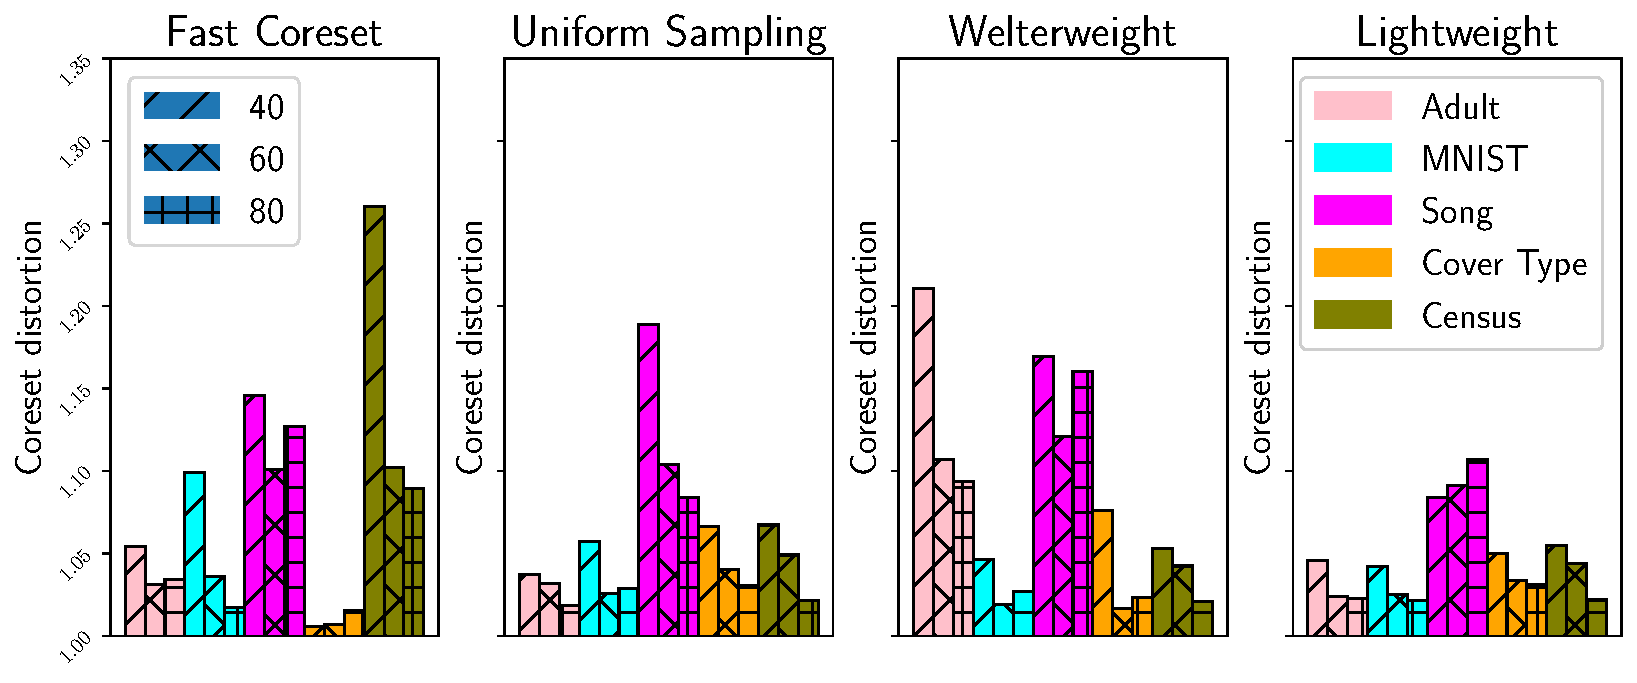
\includegraphics[width=\linewidth]{images/distortion_real_data} \\
    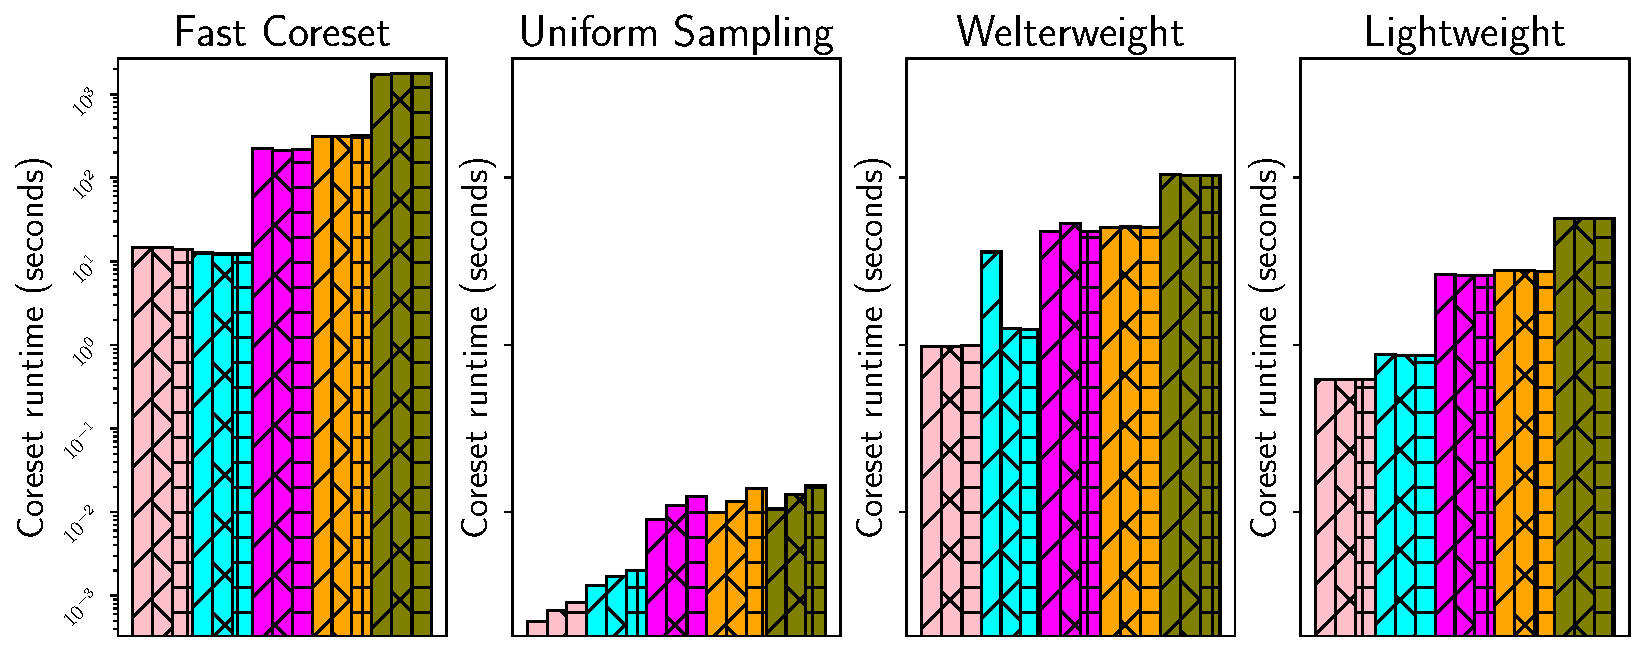
\includegraphics[width=\linewidth]{images/runtime_real_data}
\end{tabular}

\caption{\emph{Top}: The effect of the $m$-scalar on coreset distortion for real-world datasets. This is a visualization of the data in
Table~\ref{tbl:distortion}.  \emph{Bottom}: The effect of the $m$-scalar on the algorithm runtime for real-world datasets. All values are the mean over 5 runs.
The three bars represent samples of size $m=40k, 60k, 80k$.}

\label{fig:coreset_size_on_quality}
\end{figure}


We employ several real and artificial datasets to evaluate the quality of a coreset. 

For our real-world data, we utilize the Adult~\cite{Dua:2019}, MNIST~\cite{mnist}, Song~\cite{song}, Census~\cite{census}, and Cover Type~\cite{covtype} datasets, whose characteristics are summarized in 
Table~\cref{tbl:datasets} below.
\begin{table}[htbp]
    \label{tbl:datasets}
    \centering
    \begin{tabular}{lrr}
        Dataset & Points & Dim \\
        \hline
        \emph{Adult} & 48\,842 & 14 \\
        \emph{MNIST} & 60\,000 & 784 \\
        \emph{Song} & 515\,345 & 90 \\
        \emph{Cover Type} & 581\,012 & 54 \\
        \emph{Census} & 2\,458\,285 & 68
    \end{tabular}
    \caption{Description of real world datasets}
\end{table}

To complement those, we use several artificial datasets:
\begin{itemize}
    \item \emph{c-outlier}: $n-c$ points in a single location and $c$ points placed at a large distance away, for some constant $c$.
    \item \emph{Gaussian mixture}: multivariate Gaussians with varying cardinalities arranged randomly in high-dimensional space. \david{I think we should specify precisely what dimension, how many gaussians, with what covariance matrix}
    \item \emph{Geometric}: $n/2$ points at $(1, 0, 0, \cdots)$, $n/4$ points at $(0, 1, 0, \cdots)$, and so on. \david{I put the constant equal to $1$. What did you actually use?}
    \item \emph{Benchmark}: A specific distribution of points introduced in \cite{chrisESA} as a good testbed for coreset algorithms. 
    It has the property that all reasonable solutions are of equal quality but are maximally far
            apart in the solution space.
\end{itemize}

In all real and artificial datasets, we add random uniform noise $\eta$ with $0 \leq \eta_i \leq 0.001$ in each dimension in order to make all points unique.

\subsection{Algorithm Comparisons}
\label{ssec:alg_qualities}

\paragraph*{Comparison with standard sensitivity sampling.}
We first compare Fast-Coreset with standard sensitivity sampling, both in terms of quality and runtime. 
%verify the fact that coreset quality is independent of whether we used $k$-means++ or \fkmeans to obtain the preliminary solution. 
To this end,
Figure~\ref{fig:coreset_size_on_sens_quality} shows that, across datasets, the Fast-Coreset method produces coresets of consistent quality, with all distortion
values being lower than $1.2$ and consistently below $1.05$. \david{put the right value, for the best on each datset it should be lower}
Additionally, for sufficient coreset sizes ($m \approx 80\cdot k$), Fast-Coresets obtain similar distortion to those obtained
through sensitivity sampling. 
Despite this, Figure~\ref{fig:k_on_runtime} confirms that, while traditional sensitivity sampling runtime grows linearly with $k$,
Fast-Coreset only grow logarithmically with the number of centers. 
\david{question about this plot: what are $k$ and coreset size? It seems the legends says the first bar is for coreset size of $10k$, second one $50k$ etc. I think you told me that it is not what you did?}

 Therefore, our experimental findings confirm the theory predicted by \cref{thm:main}:
sensitivity sampling coresets can be implemented in linear time while preserving the coreset property. Given this context, we will not add traditional
sensitivity sampling to further experiments, as it is too slow to run on our large datasets and does not provide better quality results than the Fast-Coreset
method.

\paragraph*{Comparison with the other benchmark.}
We now refer the reader to Figure~\ref{fig:coreset_size_on_quality}, where we show the effect of coreset size on the distortion across datasets and methods.  We
define the coreset sizes as $|\Omega| = ck$, where $c \in [20, 40, 60, 80]$. We see that, across datasets, coresets of larger size obtain lower distortion.
First, we note that BICO performs poorly on all datasets -- even worse than uniform sampling. 
Second, uniform sampling works very poorly on the artifical datasets, and does not provide a quality below $1.15$ and the real world ones \david{add the right value}. 

We now comment on the more involved coreset constructions, lightweight and Cut-$k$-means. 
The Cut-$k$-means coreset surprisingly does not perform better than lightweight. Our tentative explanation for this lies in the reason why lightweight performs greatly on some dataset: those are rather uniform instances, well spread around their means, with clusters of equivalent sizes. \david{not sure it is true}
Sampling according to distance to the mean makes therefore sense, while sampling according to a $j$-means solution (for small $j$) actually introduces bias against points close to the centers of that solution.
 Furthermore, lightweight coreset performs bad when there are $k$ unbalanced clusters, as illustrated in the gaussian-mixture dataset, as in Figure~\ref{fig:lightweight_breaks}.
Our artificial dataset emphasize this effect, which does not appear in the real-world dataset (probably due to our choice of large $k$) but is very plausible.
\david{add precise comments, depending on the actual precision of the coreset, especially for lightweight. }

%However, it is also clear that uniform, lightweight, and Cut-$k$-means coresets (with $j=\log k$) \david{Is this the right value of $j$?} all fail on the geometric-progression and Gaussian-mixture datasets. Additionally, uniform sampling expectedly fails on the $1$-outlier problem.

\paragraph*{Additional evaluation on imbalanced clusters.}

\begin{table}[htbp]
    \label{tbl:class-imbalance}
    \centering
    \begin{tabular}{lcr}
        Algorithm & $\gamma = 0$ & $\gamma = 5$ \\
        \hline
        Lightweight Coreset & 1.2$\pm$ 0.0 & 415.6 $\pm$ 6.8 $\times 10^5$ \\
        Cut-$k$-means; $j=2$ & 2.2$\pm$1.2 & 3.5$\pm$5.8 \\
        Cut-$k$-means; $j=\log k$ & 1.6$\pm$0.9 & 3.6$\pm$7.7 \\
        Cut-$k$-means; $j=\sqrt{k}$ & 2.8$\pm$5.8 & 79.6$\pm$2.3 \\
        Fast Coreset & 1.2$\pm$0.0 & 1.3$\pm$0.0
    \end{tabular}
    \caption{The effect of $\gamma$ in the Gaussian mixture dataset on the coreset distortion. We report the means and variances over 5 random dataset generations.
    Each generation had 50\,000 points in 50 dimensions, with 10 Gaussian clusters and coresets of size 2\,000. We set $k=100$.}
\end{table}
\david{Say what is the coreset size. Do you know why is Fast Coreset so bad as well? Would it be possible to increase it to have a good fast coreset?}

As discussed, the sensitivities for lightweight coresets are obtained by a linear combination of a uniform distribution and each point's relative
distance to the mean. Since the Gaussian mixture dataset has randomly distributed clusters of varying sizes, a small cluster that is close to the mean is unlikely
to ever be sampled. We argue that, although this is a toy dataset, one can easily imagine real-world datasets that have this property. 
As a simple solution, we see
that the Cut-$k$-means coreset obtains satisfactory solutions on the Gaussian mixture dataset for 
\david{I don't know what you meant unfortunately}

A similar argument can be made for the more-challenging geometric dataset, where the cluster size decreases exponentially and all clusters are equidistant.
We show furthermore that, for small values of $j$, sensitivities obtained according to
solutions for $j$-means are insufficient to create a coreset for the geometric-progression dataset.

To measure further the effect that the class imbalance has on the quality of each coreset, we define a class imbalance parameter $\gamma$ and obtain each
cluster's size by $|C_i| = \frac{n}{m} \exp \left( \gamma(\rho - \frac{1}{2}) \right)$, where $\rho$ is distributed uniformly at random in the range $[0, 1]$. \david{is it $\rho_i$ rather?}
Thus, each cluster has size $\frac{n}{m}$ when $\gamma = 0$ and the cluster sizes diverge exponentially as $\gamma$ grows linearly. We see the effect of $\gamma$ on the coreset
distortion in Table~\ref{tbl:class-imbalance}, where even small values of $\gamma$ can break the lightweight coreset construction.
\david{the sentence "cluster sizes diverge exponentially as $\gamma$ grows linearly" is not super clear to me, because of the randomness. Also, since you are only showing two values of $\gamma$, it is hard to say that "it grows linearly": would it be possible to add the ratio max size / min size for $\gamma = 5$ ? This should be something close to $\exp(10)$ which is crazy huge compared to $50000$, so maybe not the right thing to plot...}
 Looking at the
sensitivities computed via $j$-means++, we see that using $(j>1)$ is better at maintaining the coreset property for higher values of $\gamma$ but is still not guaranteed
to obtain satisfactory compression. Despite this, sensitivity sampling consistently obtains coresets with low distortion. 
\david{The description of the dataset does not match the table's caption: are you sure there are 50 000 points? Also, need to be more precise: what are the mean / variance of gaussians? }

Lastly, we employ the \emph{Benchmark} dataset that  as a particularly challenging problem for coreset constructions.  The
benchmark dataset is  This naturally stress-tests
the sensitivity sampling approach, as every candidate solution's sensitivities are particularly difficult to approximate. \david{not sure we need to say more than in section 3.1.3 and in the paragraph explaining Figure~\ref{fig:coreset_size_on_quality}}

\begin{figure*}
\label{fig:coreset_size_on_sens_quality}
\centering
\begin{tabular}{lc}
    \rotatebox[origin=l]{90}{\bf \;\quad\quad\quad\quad\quad\quad\quad$k$-Median} &
    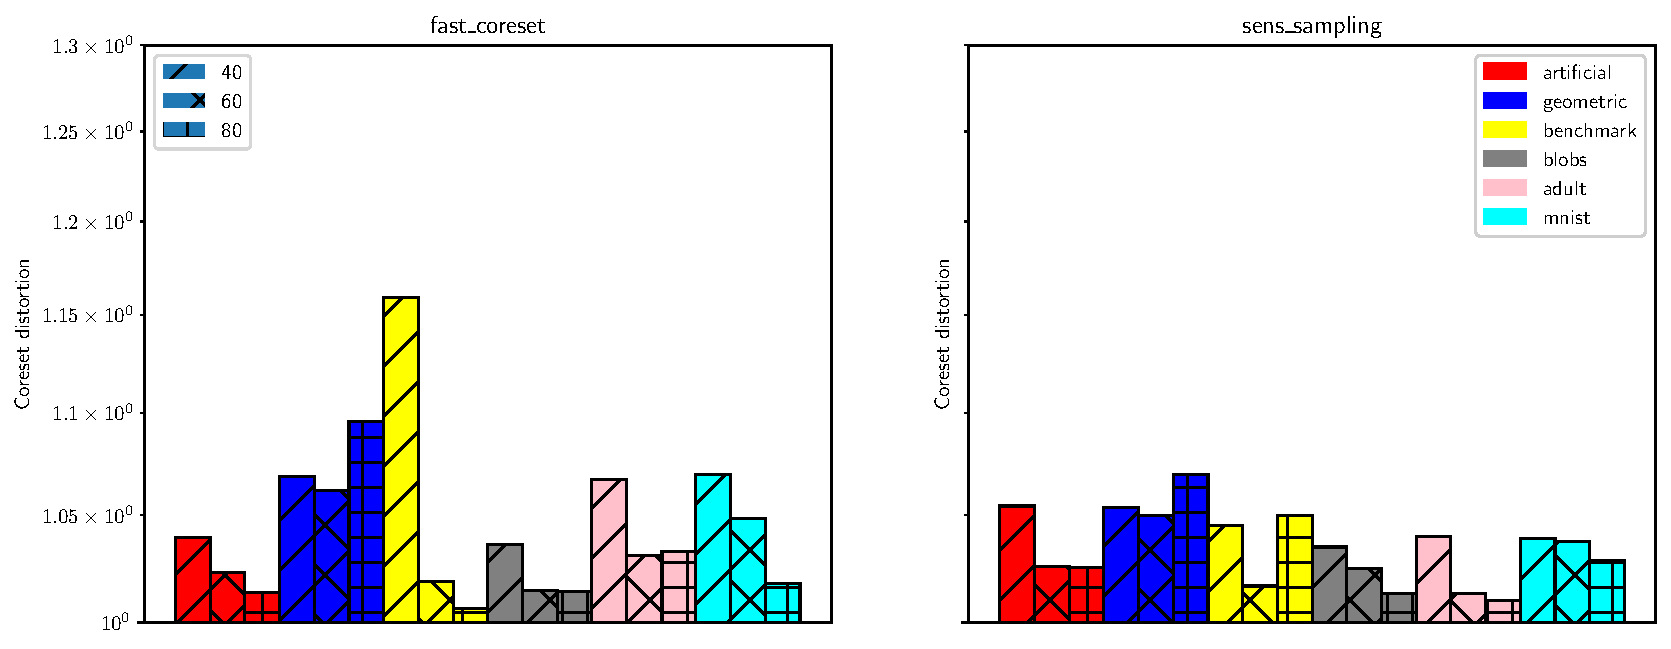
\includegraphics[width=.95\linewidth]{images/1/coreset_distortion-m_scalar_for_sens_sampling.pdf} \\

    \rotatebox[origin=l]{90}{\bf \;\;\quad\quad\quad\quad\quad\quad\quad$k$-Means} &
    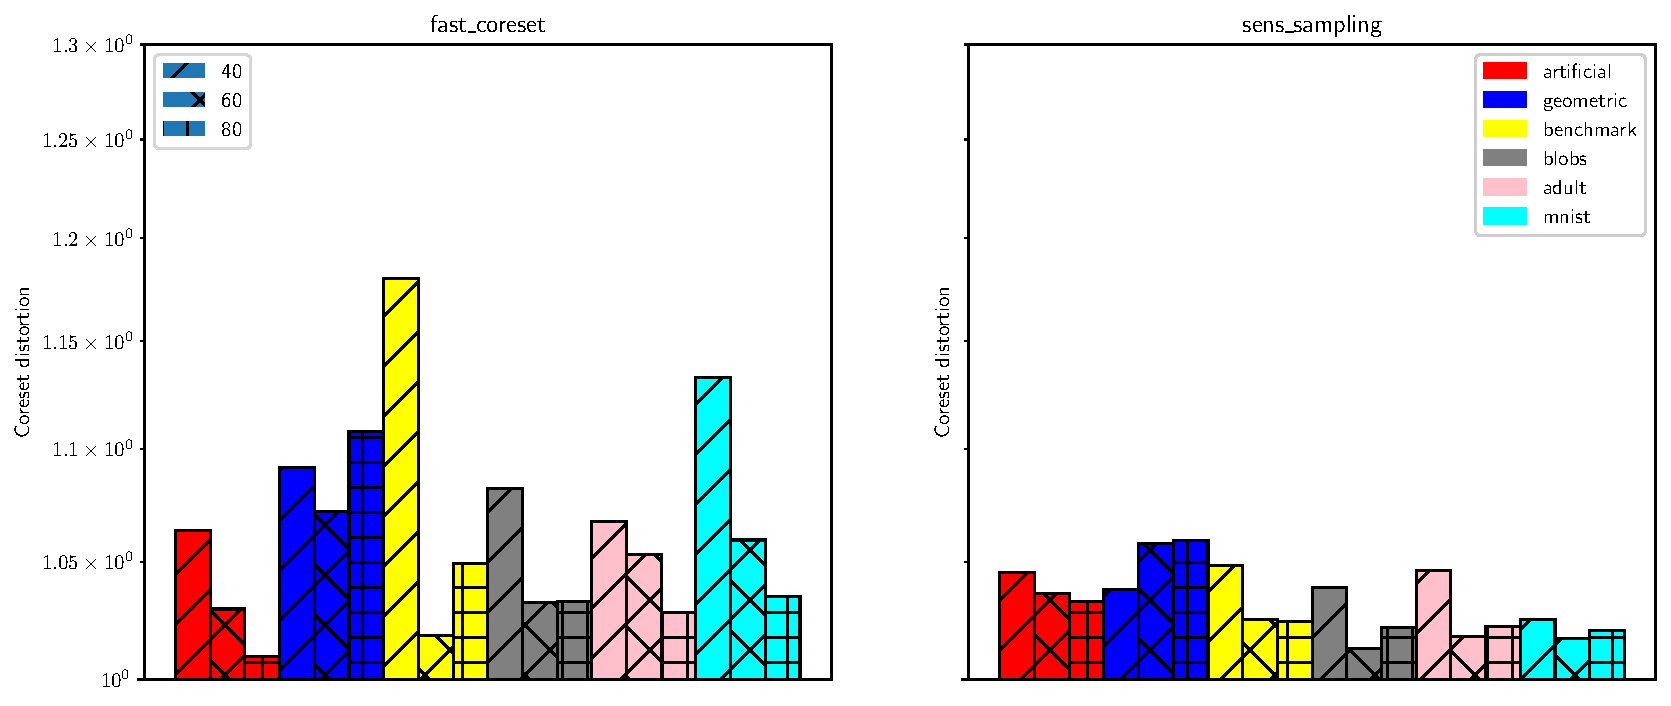
\includegraphics[width=.95\linewidth]{images/2/coreset_distortion-m_scalar_for_sens_sampling.pdf}
\end{tabular}
\caption{The effect of the coreset size on the distortion metric for sensitivity sampling approaches.
We point out that all distortion values are well below $\varepsilon = 0.2$.
Thus, for sufficient coreset sizes, there does not seem to be a meaningful difference between using Fast-Kmeans++ vs. regular Kmeans++.}
\end{figure*}

\begin{figure*}
    \centering
    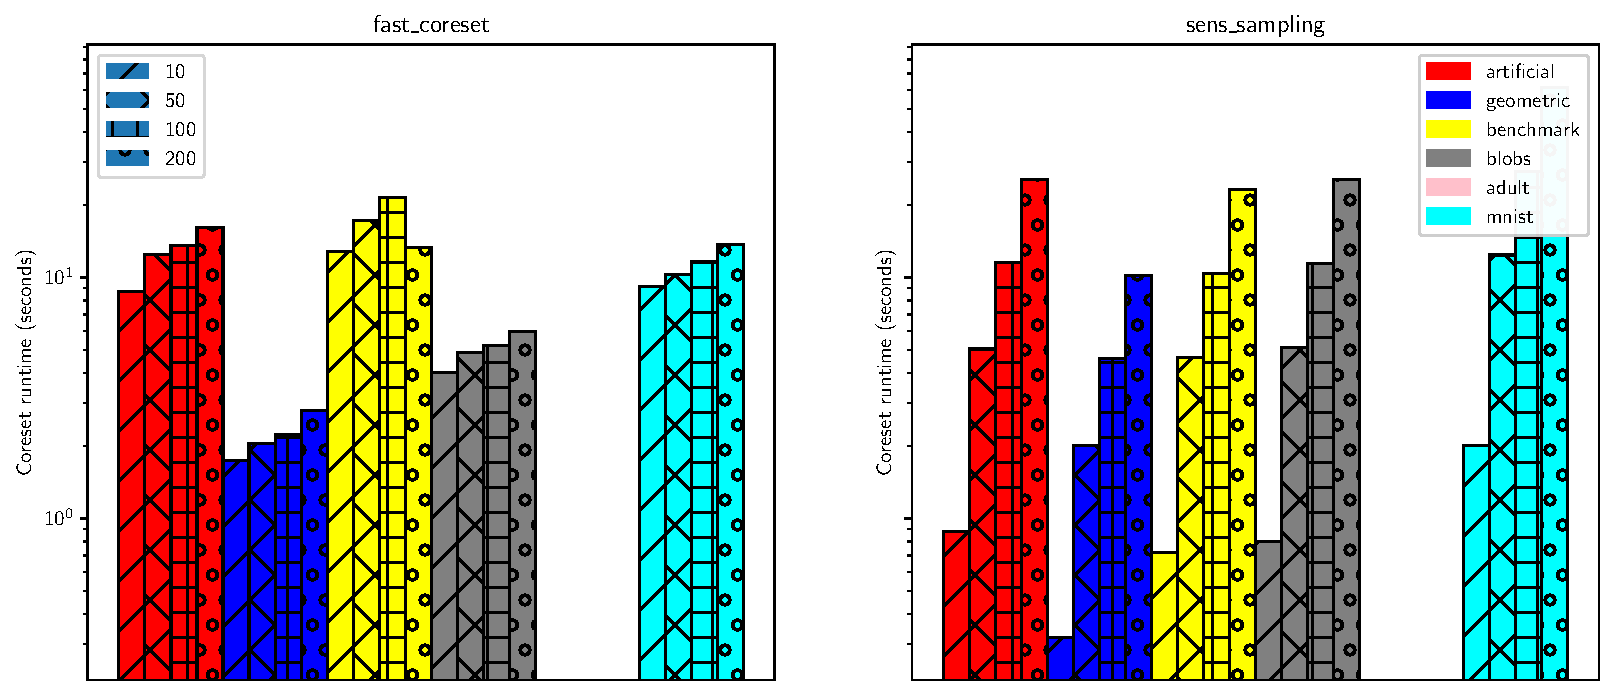
\includegraphics[width=.95\linewidth]{images/2/coreset_runtime-Effect_of_k_for_sens_sampling.pdf}
    \caption{
        The effect of $k$ on the coreset algorithm runtime. We see that traditional sensitivity sampling grows linearly with $k$ while Fast-Kmeans++ grows
        logarithmically.
    }
    \label{fig:k_on_runtime}
\end{figure*}

\begin{figure*}
\label{fig:lightweight_breaks}
\centering
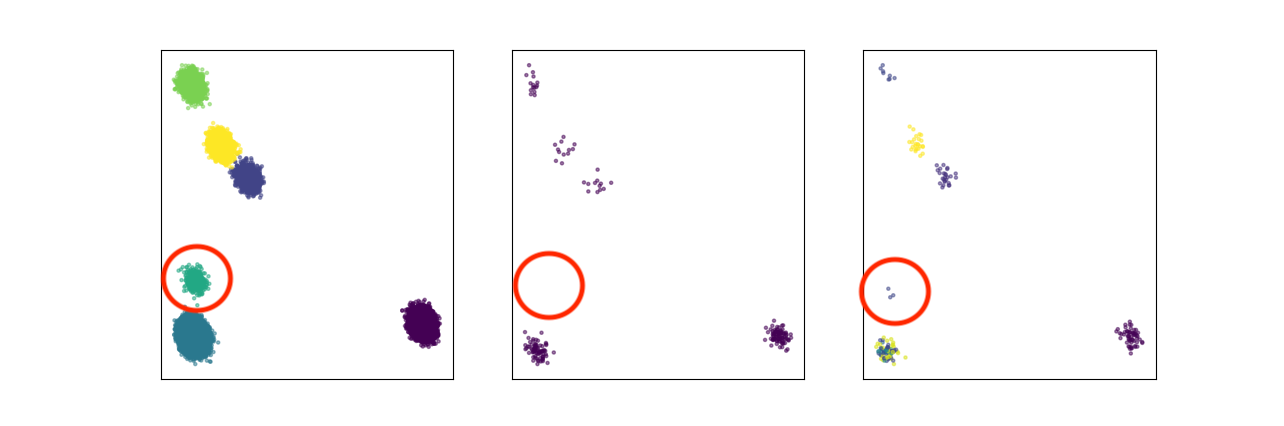
\includegraphics[width=.95\linewidth]{images/lightweight_breaks.png}
\caption{
The results of lightweight and fast-coreset constructions on a dataset of $n=100K$ points with clusters of varying size. Coresets have 200 points.
\emph{Left}: Original multivariate-Gaussian dataset. \emph{Middle}: Lightweight coresets fail to capture the cluster of $\sim$400 points.
\emph{Right}: The Fast-coreset construction runs in linear time but identifies all of the clusters.
}
\end{figure*}

